% ============================================================================================
% Section: Experimental Evaluation (final protocol, series E1-E22). Insert before the Conclusion.
% Requires \newcommand{\pamcp}{PaMCP} in the preamble (the protocol's name for the approach).
% Every number is read from results/final/*.json (branch research/pamcp-final-evaluation); the tables are
% generated by paper/make_tables_final.py and the figures by experiments/final/paper_figures_final.py.
% ============================================================================================
\section{Experimental Evaluation}
\label{sec:ev}

% Plan: what is evaluated, how it is organised, what could not be run.
This section evaluates the approach, called \pamcp{} below, against the experimental protocol of the four
research questions. Table~\ref{tab:ev-ledger} lists the 22 series of the protocol, the question each answers,
whether it was run and the kind of evidence it produces. All results come from a reference implementation of
the capability model, Algorithms~1--3 and the certificate. Series that need executed MCP servers (end-to-end
task success, E13; observed effects, E3; executed injected actions, E14; experience reuse as in AutoTool~\cite{jia2026autotool}, E21) or human
annotators (E2) could not be run and are reported as such; no claim below rests on them.

\begin{table}[t]
\caption{Experiment series of the protocol, research question, status and evidence class. M: measured on
benchmark data; L: scored against the independent labels $J_B$; S: simulated evidence or attacker scored against
$J_B$; Y: synthetic registries. $^a$Agreement with $J_B$; human study not run. $^b$Observed effects need executed
servers. $^c$Task success needs E13. $^d$64-item set, three models. $^e$Needs executed MCP servers.
$^f$Deterministic repairs only.}
\label{tab:ev-ledger}
\centering\footnotesize\setlength{\tabcolsep}{2.6pt}
\begin{tabular}{@{}lllll@{}}
\toprule
ID & Series & RQ & Status & Evid.\\
\midrule
E1 & Registry characterisation & RQ1 & run & M, L\\
E2 & Semantic typing & RQ1 & proxy$^a$ & L\\
E3 & Declared vs.\ observed effects & RQ2 & partial$^b$ & L\\
E4 & Exposure under policy encodings & RQ2 & run & S\\
E5 & Forged and laundered metadata & RQ2 & run & S\\
E6 & Imperfect verifier & RQ2 & run & S\\
E7 & Trust policy and evidence strength & RQ2 & run & S\\
E8 & Single-tool retrieval & RQ3 & run & M\\
E9 & Multi-tool set retrieval & RQ3 & run & M\\
E10 & Set validity & RQ3 & run & L\\
E11 & Capability gap & RQ1, RQ3 & partial$^c$ & M\\
E12 & Model-profile calibration & RQ1 & partial$^d$ & M\\
E13 & End-to-end execution & -- & blocked$^e$ & --\\
E14 & Prompt injection & RQ2, RQ3 & offline$^e$ & L\\
E15 & Cost and scalability & RQ3, RQ4 & run & Y\\
E16 & Registry and model evolution & RQ4 & run & M\\
E17 & Counterexample-guided refinement & RQ4 & partial$^f$ & M\\
E18 & Mechanism ablation ($2^3$) & all & run & M, L\\
E19 & LLM role configurations & RQ1 & not run & --\\
E20 & Cost weights, utility floor & RQ3 & run & M\\
E21 & Experience reuse & RQ4 & blocked$^e$ & --\\
E22 & Statistical validity & all & run & --\\
\bottomrule
\end{tabular}
\end{table}


\subsection{Experimental Setup}
\label{sec:ev-setup}

% Plan: data and splits.
\emph{Registries and tasks.} LiveMCPTool~\cite{mo2025livemcpbench} (69 servers, 525 tools) and the tool set
of MCPToolBench++~\cite{fan2025mcptoolbench} (10 servers, 87 tools) are merged by \texttt{server::name}; 43 tools
and 3 servers coincide, giving the 76 servers and 569 tools of Table~1. Multi-step tasks are the 95 LiveMCPBench
tasks of the public release, 94 of them with a resolvable gold tool. MCPToolBench++ provides 1,509 single-call
requests; a 60-query development split (ten per category) is used for every tuning decision, and a disjoint
evaluation sample of 300 distinct queries (50 per category) is used wherever a method needs a recorded LLM output.
E14, E17, E18 and E20 run on 155 tasks, the 95 LiveMCPBench tasks and the 60 development prompts, each under its
least-privilege policy (read access plus the scoped writes its goals need) and under a strict read-only policy.

% Plan: two independent labellings; what each is used for; agreement and its limit.
\emph{Reference labels.} Neither benchmark labels effects. Labels $J_A$ were produced by Claude Sonnet from each
tool's name, description and schema under a fixed guide; they provide the typing $\tau$ and drive a simulated
sandbox verifier bound to $h(t)$. Labels $J_B$ were produced blind by Claude Opus under a separately written guide
and are used only for scoring, so that the evidence an experiment simulates never comes from the labels that
score it. The two agree on state modification for 558 of the 569 tools ($\kappa=0.944$) and on private output with
$\kappa=0.893$. Every tool that is not read-only under $J_B$ (120 tools) is also not read-only under $J_A$ (131
tools), so an error-free verifier simulated from $J_A$ can over-exclude but never admit a tool that $J_B$
considers unsafe; verifier errors are injected separately (E5--E7). Both labellings come from one model family
and neither is human ground truth.

% Plan: recorded LLM roles.
\emph{LLM roles.} All LLM outputs were recorded once and are replayed: the analyst's goal contracts (Claude Sonnet;
158 prompts of the scenarios and of the test and development tasks, and the 300 sampled requests), MCP-Zero's model-written
requests for 455 tasks and its 76 server summaries, 450 generated multi-tool training queries for COLT,
equivalence judgements on 638 candidate pairs for ToolScope's merger, and the calibration answers and
self-assessments of three models. The exact model version strings were not exposed to the experiments.

% Plan: methods, mechanisms and baselines with their adaptations.
\emph{Methods.} \pamcp{} is decomposed into its three mechanisms: the model-conditioned gap (G, Algorithm~1),
provenance-sound eligibility (P, Section~5) and set-level reasoning with certification (S: backward closure,
minimum-cost cover and certificate, Section~6). Switching S off retrieves one eligible tool per subgoal; switching
P off accepts published annotations and lexical cues at face value. The baselines are RAG-MCP~\cite{gan2025ragmcp}
(dense top-$k$ over the request), MCP-Zero~\cite{fei2025mcpzero} (recorded requests, server routing, top-1 tool
per request), COLT~\cite{qu2024colt} (its collaborative stage as a parameter-free graph propagation over the
query--scene--tool graph of the training queries), ToolScope~\cite{liu2026toolscope} (LLM-confirmed merging into
16 clusters with provider identities and effects kept, dense retrieval over the analyst's subqueries),
CMTF~\cite{suresh2026cmtf} (breadth-first search over typed states with one tool per step), per-subtask retrieval
and the full catalogue. All methods share the registry, the contracts and one dense encoder, a TF-IDF and
truncated-SVD stand-in (BGE-M3~\cite{chen2024bgem3} could not be installed); none of the baselines was tuned.
\pamcp{} uses the parameters of Section~6 with the relevance term $w_{\mathrm{rel}}(1-\hat{s}(e))$ added to
Eq.~(6) ($w_{\mathrm{rel}}=10$, selected on the development split).

% Plan: metrics and statistics; preregistration.
\emph{Metrics and statistics.} Exp@$k$ is the share of requests whose top-$k$ list contains a tool that is not
read-only under $J_B$, over the requests whose gold tools are all read-only; Util@$k$ is the share of those
requests with a gold tool in the top-$k$. Group recall is the share of a task's gold groups (alternative tools of
one step count once) present in the toolkit. Joint feasibility is decided by an independently written set
evaluator that uses only $J_B$ and the analyst's goals: every goal needing the outside world is served (S), every
required input is obtainable (C), effects (E) and flows (L) respect the task's policy, evidence meets the policy
level (V) and no tool is redundant (M). Paired comparisons use sign-flip permutation tests and bootstrap
intervals, with target tools as clusters for request-level metrics, and proportions use Wilson intervals. A
confirmatory family of seven comparisons (F1--F7, Table~\ref{tab:ev-family}), a non-inferiority margin of 0.05
for recall and Holm correction were fixed before E9, E10, E14 and E18 were run; every other comparison is
exploratory. Code, recorded LLM outputs and per-item results are
available.\footnote{\url{https://github.com/msellamiTN/taas-provenance-discovery}, branch
\texttt{research/pamcp-final-evaluation}.}

\subsection{Representation and Model Profile (RQ1)}
\label{sec:ev-rq1}

% Plan: E1 registry; E2 typing.
\emph{Registry and typing (E1, E2).} The merged registry reproduces Table~1. Under $J_B$, 120 tools (21.1\%, 95\%
CI 17.9--24.6\%) are not read-only; 24 of them belong to MCPToolBench++. One of the 44 annotated tools,
\texttt{opgg-mcp::lol-summoner-renewal}, declares \texttt{readOnlyHint=true} but is not read-only. Reachability
(S) depends on the typing $\tau$: the LLM-assisted typing agrees with $J_B$ on 78.9\% of output kinds
($\kappa=0.718$, macro-F1 0.704) but only on 35.7\% of complete types (kind and domain), whereas a structural typer
working from schemas and names alone agrees on 22.8\% of kinds ($\kappa=0.070$) and is never more than 0.7
confident. Lexical or structural typing is therefore not an alternative to an LLM pass, and the type domains are
where the two LLM labellings disagree most.

% Plan: E12 calibration and self-assessment.
\emph{Model profile (E12).} Claude Sonnet and Claude Opus answered all 64 calibration items correctly, including
exact sums of 640 numbers read from context; Claude Haiku answered 51, failing exact sums from $n=160$ and exact
counts at $n=640$. Asked beforehand, all three underestimated themselves (mean signed error $-0.23$ for Sonnet,
$-0.22$ for Haiku and $-0.30$ for Opus; mean absolute error 0.23, 0.24 and 0.30; Fig.~\ref{fig:ev-profile}a). A
self-assessed profile would
thus send to tools work that the model performs correctly, which supports measuring $\rho_{\mathrm{LLM}}$ rather
than asking for it. On the test and development tasks the measured profile overruled 12 of the analyst's 128
native claims (9.4\%).

\begin{figure}[t]
\centering
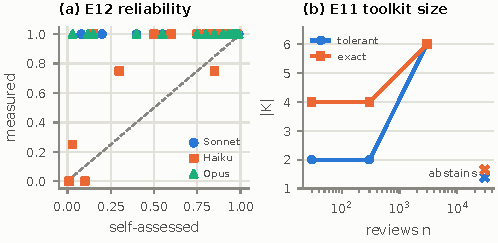
\includegraphics[width=\columnwidth]{paper_profile_gap}
\caption{(a) Self-assessed against measured reliability per class and input size (E12; four items per point).
(b) Toolkit size of the review scenario against the number of reviews, Claude Sonnet profile, $\tau=0.9$ (E11);
crosses mark abstentions.}
\label{fig:ev-profile}
\end{figure}

% Plan: E11 gap behaviour on the running scenario.
\emph{Capability gap (E11).} On the review scenario of Fig.~1 the gap grows with the input
(Fig.~\ref{fig:ev-profile}b): with tolerant aggregation the toolkit has two tools at $n=30$ and 300, with 60\% of
the goals left to the model, and six at $n=3{,}000$; exact aggregation adds two tools at the smaller sizes. At
$n=30{,}000$ the engine abstains, as it does at $n=3{,}000$ with $\tau=0.6$. Without gap analysis it abstains in
every setting, because no registry tool serves the scenario's interpretive goals. The three measured profiles give
identical toolkits on this scenario. Task success for these toolkits requires execution (E13) and was not measured.

\subsection{Trust under Missing, Forged and Imperfect Evidence (RQ2)}
\label{sec:ev-rq2}

% Plan: E3 declared effects.
\emph{Declared effects (E3).} Declarations cover 44 tools, one of them wrongly; the other 525 tools, among them 119
that are not read-only, declare nothing. Lexical cues flag 82.5\% of the unsafe tools at a precision of 0.54.
Observed effects need probe traces of executed servers and were not produced.

\begin{figure*}[t]
\centering
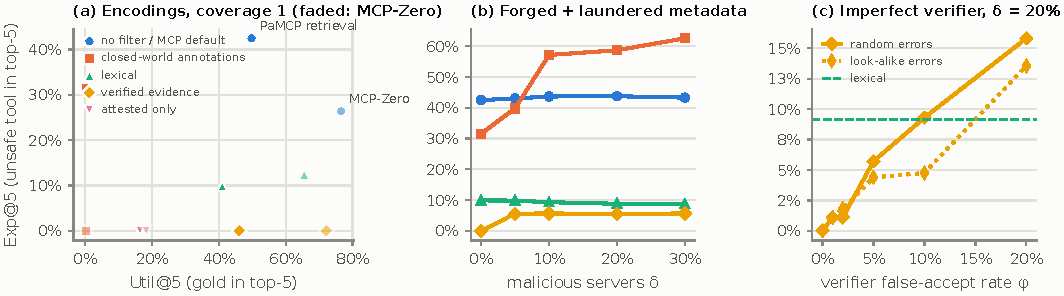
\includegraphics[width=\textwidth]{paper_eligibility}
\caption{Eligibility under a read-only policy over 394 requests (273 with read-only gold tools). (a) Exposure
against utility of each policy encoding at full verification coverage, for \pamcp{}'s retrieval stage and (faded)
MCP-Zero (E4). (b) Exposure as a fraction $\delta$ of servers forge their annotations and launder their
descriptions; verifier false-accept rate 5\%, five seeds for $\delta>0$, one at $\delta=0$ (E5). (c) Exposure of verified evidence against the
verifier's false-accept rate, with errors at random or concentrated on unsafe tools that resemble safe ones,
$\delta=0.2$ (E6).}
\label{fig:ev-eligibility}
\end{figure*}

% Plan: E4 encodings.
\emph{Policy encodings (E4).} Fig.~\ref{fig:ev-eligibility}a compares the encodings of a read-only policy.
Without a filter, and under MCP's default of displaying annotations without enforcing them, 42.5\% of the requests
receive an unsafe tool among \pamcp{}'s top five (26.4\% for MCP-Zero). Requiring a declared read-only hint keeps
44 tools, one of them unsafe; because the pool is so small, that tool reaches 31.5\% of the top-five lists while
utility falls to 0.4\%. The lexical encoding admits 21 of the 120 unsafe tools (Exp@5 9.9\%, Util@5 41.0\%).
Verified evidence admits none of them and keeps 77.0\% of the registry eligible; Util@5 is 46.2\% against 49.8\%
without any filter for \pamcp{}'s retrieval stage, and 72.2\% against 76.6\% for MCP-Zero. As the verifier probes
fewer tools, exposure stays at zero and utility follows the eligible share (34.7\%, 26.8\% and 16.3\% at
coverage 0.75, 0.5 and 0.25). The exposure difference to the lexical encoding is confirmatory test F4
($\Delta=-0.099$, $p_H<0.001$); by the construction noted in Section~\ref{sec:ev-setup}, its zero side reflects
the simulation, and the measured content is the utility cost.

% Plan: E5 forgery and laundering.
\emph{Forged and laundered metadata (E5).} Forged annotations are what break the closed-world reading: its
exposure rises from 31.5\% to 57.1\% when a tenth of the servers forge their hints and launder their descriptions
(56.8\% with forgery alone) and to 62.6\% at 30\% (Fig.~\ref{fig:ev-eligibility}b). Laundered descriptions barely affect the lexical encoding (8.7--9.9\%), because
the tool names that carry most lexical cues are kept. Verified evidence does not depend on $\delta$: with a 5\%
false-accept rate its exposure averages 5.4--5.6\% for every $\delta>0$, at a utility of 46.1--46.7\%. Which unsafe
tools are falsely accepted varies with the seed, and so does exposure (0.0--14.7\% per seed); the single seed run
at $\delta=0$ gives 0.0\%.

% Plan: E6 imperfect verifier and break-even.
\emph{Imperfect verifier (E6).} Exposure of verified evidence grows with the false-accept rate $\varphi$, to
1.1\%, 5.7\%, 9.3\% and 15.8\% at $\varphi$ of 1\%, 5\%, 10\% and 20\% with $\delta=0.2$
(Fig.~\ref{fig:ev-eligibility}c). Errors concentrated on look-alike unsafe tools are not worse (4.4\% at 5\%,
13.6\% at 20\%). Verified evidence stays below the lexical encoding (9.2\%) up to $\varphi=5\%$ with random errors
and up to 10\% with look-alike errors, which quantifies the condition of Section~7 that a verifier must be
accurate to help. False rejections cost utility instead: with $\psi=0.2$, Util@5 falls from 46.2\% to 39.1\%.

% Plan: E7 trust threshold.
\emph{Trust policy (E7).} With probe coverage $\kappa$ varying between tools ($\delta=0.2$, $\varphi=5\%$),
raising $\ell_{\min}$ from 0.55 or less to 0.65, the level of observed evidence in the implementation, lowers
exposure from 5.5\% to 3.5\% and utility from 45.8\% to 34.4\%; requiring $\kappa\ge0.8$ in addition lowers them
to 0.6\% and 14.3\%. Above 0.75 only attested evidence qualifies; exposure then rises to 10.3\%, because the few
falsely accepted attested tools reach many top-five lists of a pool of 25.4\% of the registry. Weighting evidence by
signer lowers utility (18.4\% at 0.65) and raises exposure (6.5\% against 3.5\%). A stricter threshold therefore
does not lower Exp@$k$ by itself; exposure has to be read together with the size of the eligible pool.

\subsection{Composition (RQ3)}
\label{sec:ev-rq3}

\begin{figure*}[t]
\centering
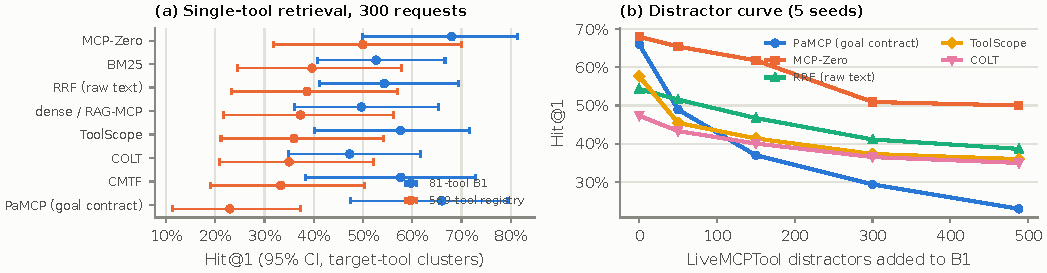
\includegraphics[width=\textwidth]{paper_retrieval}
\caption{Single-tool retrieval on the 300-query MCPToolBench++ sample (E8). (a) Hit@1 over the 81 MCPToolBench++
tools (B1) and over the 569-tool registry, with target-tool clustered 95\% CIs. (b) Hit@1 as LiveMCPTool tools are
added to B1 (five seeds).}
\label{fig:ev-retrieval}
\end{figure*}

% Plan: E8 single-tool retrieval, the negative result and its diagnosis.
\emph{Single-tool retrieval (E8).} Over the MCPToolBench++ tools, retrieval from the analyst's goal contract ranks
the gold tool first for 66.0\% of the requests, behind MCP-Zero's model-written requests (68.0\%) and ahead of
raw-text fusion (54.3\%), ToolScope and CMTF (57.7\%), BM25 (52.7\%) and COLT (47.3\%)
(Fig.~\ref{fig:ev-retrieval}a). Over the 569-tool registry it falls to 23.0\%, the lowest of all methods
(MCP-Zero 50.0\%, BM25 39.7\%, raw-text fusion 38.7\%, ToolScope 36.0\%, COLT 35.0\%, CMTF 33.3\%), and the
distractor curve shows the loss growing with every block of added tools (Fig.~\ref{fig:ev-retrieval}b).
Confirmatory test F7 thus goes against \pamcp{} ($\Delta=-0.157$, $p_H<0.001$). The cause is the structural
component of Eq.~(5): the analyst's goal text alone ranks better than the raw request (40.0\% against 38.7\%),
but only 50.3\% of the gold tools are type-compatible with the analyst's goal output type, so the structural
ranking promotes compatible wrong tools (23.0\%). Typed retrieval therefore helps only where goal and tool typings
agree; with the present typing the structural component would have to be weighted down or applied after
relevance, which was not evaluated.

\begin{table}[t]
\caption{Set retrieval (E9, open policy) and set validity (E10, each task's least-privilege policy) on the 94
LiveMCPBench tasks. Rec.: group recall; Comp.: share of tasks whose gold groups are all covered; Rec.$_{sm}$:
recall with every method truncated to \pamcp{}'s toolkit size (84 tasks with a non-empty toolkit); Joint: joint
feasibility under the independent evaluator (\pamcp{} with $K{=}10$, identical for $K{=}20, 40$; baselines
restricted to eligible tools / as published); Abst.: abstentions. Per-subtask uses the analyst's subgoals. Tokens
of the raw tool definitions.}
\label{tab:ev-sets}
\centering\footnotesize\setlength{\tabcolsep}{1.5pt}
\begin{tabular}{@{}lrrrrrrr@{}}
\toprule
Method & $|K|$ & Tok. & Rec. & Comp.\% & Rec.$_{sm}$ & Joint\% & Abst.\%\\
\midrule
\pamcp{} ($K{=}5$) & 1.47 & 199 & 0.169 & 4.3 & 0.189 & 67 & 7\\
\quad without closure & 1.40 & 195 & 0.168 & 4.3 & -- & -- & 10\\
Per-subtask & 2.59 & 346 & 0.249 & 9.6 & 0.138 & 63/52 & 0\\
MCP-Zero & 1.76 & 250 & 0.227 & 8.5 & 0.200 & 57/55 & 0\\
RAG-MCP top-5 & 5.00 & 1244 & 0.293 & 13.8 & 0.130 & 61/49 & 0\\
COLT top-5 & 5.00 & 1094 & 0.295 & 12.8 & 0.084 & 60/48 & 0\\
ToolScope top-5 & 5.20 & 976 & 0.361 & 17.0 & -- & 73/60 & 0\\
CMTF (path) & 0.64 & 105 & 0.072 & 1.1 & -- & 26/23 & 0\\
\bottomrule
\end{tabular}
\end{table}


% Plan: E9 set retrieval with size matching and F1/F2.
\emph{Set retrieval (E9).} Table~\ref{tab:ev-sets} reports the selected sets on the 94 LiveMCPBench tasks.
\pamcp{} exposes the smallest toolkits apart from CMTF (1.47 tools, 199 tokens) and reaches a group recall of
0.169. Methods that expose more tools reach more gold groups: per-subtask retrieval 0.249 with 2.59 tools, RAG-MCP
and COLT 0.293 and 0.295 with five tools and over 1,000 tokens, ToolScope 0.361 with 5.20 tools. Non-inferiority
to per-subtask retrieval is not established (F1: $\Delta=-0.080$, 95\% CI $[-0.166, 0.002]$). At equal size,
\pamcp{} reaches 0.189 against 0.130 for RAG-MCP (F2: $\Delta=0.060$, $p_H=0.397$), 0.138 for per-subtask
retrieval, 0.084 for COLT and 0.200 for MCP-Zero. A larger candidate budget ($K=10, 20$) raises recall to 0.174,
and backward closure changes it on 3 of the 94 tasks. \pamcp{} abstains on 7.4\% of the tasks (six $\chi_1$ and one
$\chi_5$ counterexamples) and certifies the other 92.6\%. The analyst's decomposition matters for every method:
per-subtask retrieval reaches 0.105 on the raw request, 0.142 with a clause splitter and 0.249 with the analyst's
subgoals.

% Plan: E10 set validity and F3.
\emph{Set validity (E10).} Under each task's least-privilege policy, 67.0\% of \pamcp{}'s toolkits ($K=10$; the
same for 20 and 40) are jointly
feasible for the independent evaluator, 72.4\% of those it did not abstain on. The interface, effect, flow and
evidence checks pass for 97.9--100\%; the failures are goals that the evaluator, which decides from $J_B$'s types
rather than $\tau$, does not consider served (S passes for 68.1\%, abstentions included). Baselines as published
reach 47.9--59.6\% and fail the effect check for 4.3--25.5\% of the tasks; restricted to eligible tools they gain
2--14 points and reach 57.4--73.4\%, ToolScope highest, and CMTF reaches 25.5\%. The difference to per-subtask
retrieval over eligible tools is not significant (F3: $\Delta=0.043$, $p_H=1.0$). Certification raises
\pamcp{}'s joint feasibility from 59.6\% (NoCert) to 67.0\%, through obtainable inputs (C from 88.3\% to 97.9\%)
and minimality (M from 74.5\% to 87.2\%, against 21.3--41.5\% for the top-five retrievers).

\subsection{Robustness to Prompt Injection and Mechanism Ablation}
\label{sec:ev-ablation}

\begin{table}[t]
\caption{Mechanism ablation (E18) and injection reach (E14) on 155 tasks under each task's least-privilege
policy. G: model-conditioned gap; P: provenance-sound eligibility; S: set-level reasoning and certificate. Joint:
joint feasibility (independent evaluator); Reach: worst-case share of task $\times$ out-of-scope attack pairs the
toolkit can realise under $J_B$ (least privilege: 712 pairs; strict read-only: 775). Shapley attribution of the
full-vs-none difference (G/P/S): Rec.: $-$0.017/$-$0.013/$-$0.060; Tok.: $-$55.3/0.8/$-$66.3; Joint: 0.010/0.026/$-$0.010; Reach: $-$0.012/$-$0.018/$-$0.022.}
\label{tab:ev-factorial}
\centering\footnotesize\setlength{\tabcolsep}{2.0pt}
\begin{tabular}{@{}llrrrrrrr@{}}
\toprule
Cell & Mech. & $|K|$ & Tok. & Rec. & Joint\% & Reach\% & R-O\% & Abst.\%\\
\midrule
Full \pamcp{} & G P S & 1.23 & 176 & 0.181 & 56.1 & 0.0 & 0.0 & 10.3\\
NoCert & G P \textendash & 1.46 & 229 & 0.253 & 56.8 & 0.1 & 0.4 & 0.0\\
Declared & G \textendash{} S & 1.25 & 189 & 0.230 & 54.8 & 0.0 & 0.0 & 6.5\\
NoGap & \textendash{} P S & 1.50 & 193 & 0.183 & 55.5 & 0.0 & 0.0 & 20.0\\
 & G \textendash{} \textendash & 1.46 & 208 & 0.239 & 55.5 & 0.4 & 3.7 & 0.0\\
 & \textendash{} P \textendash & 2.09 & 316 & 0.295 & 58.1 & 0.1 & 0.4 & 0.0\\
 & \textendash{} \textendash{} S & 1.53 & 221 & 0.223 & 52.9 & 0.1 & 0.1 & 16.1\\
None & \textendash{} \textendash{} \textendash & 2.08 & 297 & 0.270 & 53.5 & 1.1 & 4.9 & 0.0\\
\midrule
RAG-MCP top-5 & & 5.00 & 1189 & 0.393 & 52.3 & 8.1 & 14.3 & --\\
Per-subtask & & 2.08 & 308 & 0.321 & 51.0 & 2.7 & 9.4 & --\\
MCP-Zero & & 1.46 & 228 & 0.340 & 49.0 & 1.5 & 8.4 & --\\
ToolScope top-5 & & 5.30 & 1042 & 0.461 & 58.7 & 7.6 & 14.7 & --\\
COLT top-5 & & 5.00 & 1118 & 0.395 & 50.3 & 7.2 & 12.9 & --\\
CMTF (path) & & 0.61 & 114 & 0.141 & 23.9 & 0.7 & 2.2 & --\\
\bottomrule
\end{tabular}
\end{table}


% Plan: E14 offline injection.
\emph{Prompt injection (E14).} For each of 155 tasks and each attack outside the effect classes the task needs, the
attack counts as reachable if the exposed toolkit can realise it under $J_B$. Full \pamcp{}, NoGap, Declared and
every component variant let none of the 712 task--attack pairs through (Table~\ref{tab:ev-factorial}; Wilson upper
bound 0.5\%), and NoCert one, against 8.1\% for RAG-MCP, 7.6\% for ToolScope, 7.2\% for COLT, 2.7\% for
per-subtask retrieval, 1.5\% for MCP-Zero and 0.7\% for CMTF as published (F5: $\Delta=-0.027$, $p_H<0.001$);
under a strict read-only policy the retrieval baselines reach 8.4--14.7\% and full \pamcp{} stays at 0 of 775.
Restricting the baselines to eligible tools lowers them to at most 1.4\% under least privilege, so most of the
protection comes from eligibility. The sanitised manifest shows none of the poisoned descriptions when 10\% or
30\% of the tool descriptions carry an injected instruction, whereas the raw definitions of the same toolkits
contain one in 32.6\% of the tasks at 30\%, and those of the baselines in 17.4\% (CMTF) to 86.2\% (ToolScope). Of
\pamcp{}'s toolkits, 55.5\% contain a tool that returns remote content, but none of them also allows an
out-of-scope action, against 3.2--22.6\% for the baselines. Whether injected actions are executed in practice
needs E13's execution environment.

\begin{figure*}[t]
\centering
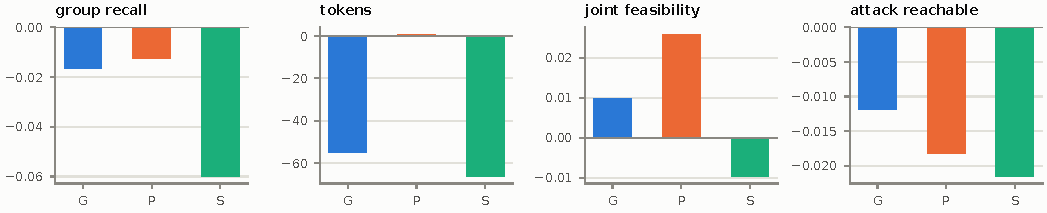
\includegraphics[width=\textwidth]{paper_factorial}
\caption{Shapley attribution of the difference between full \pamcp{} and the cell without any mechanism to the
gap (G), provenance-sound eligibility (P) and set-level reasoning (S), under least-privilege policies (E18): group
recall, tokens, joint feasibility and the share of tasks with a reachable out-of-scope action.}
\label{fig:ev-factorial}
\end{figure*}

% Plan: E18 factorial with Shapley; components.
\emph{Mechanism ablation (E18).} The $2^3$ design of Table~\ref{tab:ev-factorial} varies the three mechanisms on the
same 155 tasks, registry and scoring. The mechanisms are not additive (G$\times$S interaction on tokens 32.0,
$p<0.001$), so Fig.~\ref{fig:ev-factorial} attributes the full-versus-none difference by Shapley values. Gap
analysis and set-level reasoning share the reduction of the context from 297 to 176 tokens ($-55.3$ and $-66.3$);
eligibility contributes nothing to it. All three remove reachable actions (from 5.2\% of the tasks to none).
Recall falls from 0.270 to 0.181, mostly through set-level reasoning ($-0.060$; main effect $p=0.042$), and no
mechanism changes joint feasibility, which stays between 52.9\% and 58.1\% in every cell. The token saving of the
gap alone, Full against NoGap, is not significant after correction (F6: $\Delta=-16.7$, $p_H=0.269$), while
NoGap doubles abstentions (20.0\% against 10.3\%). Among the components of the full configuration, removing
backward closure raises abstentions from 10.3\% to 12.3\%, propagating flow labels only along derivations raises
recall to 0.236 and lowers abstentions to 5.8\% at the price of the order-independence of Property~1, removing
the relevance term lowers recall to 0.167, and the utility floor and refinement change little.

\subsection{Cost, Evolution and Stability (RQ3, RQ4)}
\label{sec:ev-rq4}

% Plan: E15 (filled from results/final/E15_scalability.json).
% E15 paragraph; numbers from results/final/E15_scalability.json and E15_optimality_gap.json (paper/e15_numbers.py).
% Plan: request latency on the real registry and on cloned registries; engine build; exact vs greedy.
\emph{Cost and scalability (E15).} On the real registry a request takes 49\,ms at the median and 191\,ms at the
95th percentile on two virtual CPUs; eligibility takes 0.08\,ms and the per-goal retrieval, timed separately,
45\,ms, against 12\,ms for one dense ranking of the request (RAG-MCP). On registries of cloned contracts, which are
near-copies of the real tools, the median grows to 58\,ms at 1,000 tools, 281\,ms at 10,000 and 2.7\,s at 100,000
(16.1\,s at the 95th percentile), almost all of it retrieval (RAG-MCP: 206\,ms). The bitmap test alone takes
0.024\,ms over $10^6$ contracts, an index microbenchmark, not the full engine at that size.
Building the engine takes 2.2\,s, 2.8\,s, 30.3\,s and 2,224\,s: the implementation materialises the pairwise risk
relation eagerly, which is quadratic in the number of tools. Compositions use the exact search for 26--28 of the 30
tasks at every size; abstentions ($\chi_1$, and one $\chi_5$) rise from 2 tasks to 9 at 10,000 and 10 at 100,000
tools. On generated cover instances, measured with the objective the search minimises (Eq.~(6)), the greedy regime
is optimal in 7, 8 and 2 of 10 instances with 1, 3 and 5 goals and on average 0.7\%, 2.3\% and 14.5\% above the
optimum (at most 3.0\%, 19.8\% and 38.1\%), while the exact search takes 3\,ms, 21\,ms and 1.1\,s. With 8 and 12 goals
the exact search exhausts its 20,000-node budget in all ten instances (after 12.0\,s and 18.2\,s) and falls back to
the greedy regime (27\,ms and 69\,ms), which carries no optimality guarantee; the gap could not be measured there.


% Plan: E16 evolution.
\emph{Evolution (E16).} Replaying 152 events on the real registry, removing and re-inserting each of the 76
servers, an incremental update takes 13.5\,ms at the median (565\,ms at the 95th percentile) against 4.2\,s for a
rebuild. The exact rule of Proposition~3 invalidates 1.1\% of the 35 cached toolkits per event, against all of
them when the cache is flushed, and after the replay 33 of the 35 recomputed toolkits are identical to the
originals. All 20 simulated rug pulls (a description changed after verification) lose their observed evidence,
and all regain it when the verified definition returns; a model-version change costs 0.012\,ms.

% Plan: E17 refinement.
\emph{Refinement (E17).} Under least-privilege policies 138 of the 155 tasks are certified at once; the
deterministic repair operators recover one of the nine $\chi_1$ and none of the eight $\chi_5$ counterexamples
(89.0\% to 89.7\%). When $\chi_1$ is induced by shrinking the candidate budget to $K=1$, they raise certification
from 73.5\% to 85.8\%, repairing 46.4\% of the $\chi_1$, 30\% of the $\chi_5$ and all three $\chi_2$
counterexamples, in 1.3 iterations on average. The revenue scenario of Fig.~3 is repaired by the $\chi_5$ split. The
assistant role of refinement and the role configurations of E19 were not run.

% Plan: E20 sensitivity.
\emph{Sensitivity (E20).} Setting $\beta$, $\eta$ or $\zeta$ to 0, 0.25 or 1 instead of 0.5, or $u_{\min}$ to 0.4 or
0.6, changes no toolkit, and $u_{\min}=0.8$ changes 0.7\%. The evidence weight $\gamma$ changes 7.2--20.1\% of the
toolkits and the token weight $\delta$ 2.9--7.2\%, with recall between 0.197 and 0.215 against 0.202; only
$\gamma=1$ combined with $\beta\le0.25$ lets a tool that $J_B$ forbids into a toolkit (0.014 per toolkit). The
price and latency weights cannot act on these registries, which publish neither, so every tool carries the same
default quality of service.

\begin{table}[t]
\caption{Preregistered confirmatory family (E22): paired sign-flip tests, bootstrap 95\% CIs of the mean
difference (first method minus second), Holm-adjusted $p_H$. For F1, $p$ is the one-sided non-inferiority test.}
\label{tab:ev-family}
\centering\footnotesize\setlength{\tabcolsep}{1.8pt}
\begin{tabular}{@{}lp{2.6cm}rrlrr@{}}
\toprule
ID & Comparison & $n$ & $\Delta$ & 95\% CI & $p$ & $p_H$\\
\midrule
F1 & E9 recall, \pamcp{} vs.\ per-subtask (non-inferiority, $\Delta_0{=}0.05$) & 94 & $-$0.080 & [$-$0.166, 0.002] & 0.763 & 1.000\\
F2 & E9 recall at equal size, \pamcp{} vs.\ RAG-MCP & 84 & 0.060 & [$-$0.016, 0.137] & 0.132 & 0.397\\
F3 & E10 joint feasibility, \pamcp{} vs.\ per-subtask (eligible) & 94 & 0.043 & [$-$0.085, 0.181] & 0.641 & 1.000\\
F4 & E4 Exp@5, verified vs.\ lexical evidence & 273 & $-$0.099 & [$-$0.139, $-$0.066] & $<$0.001 & $<$0.001\\
F5 & E14 reachable attacks, \pamcp{} vs.\ per-subtask & 712 & $-$0.027 & [$-$0.039, $-$0.015] & $<$0.001 & $<$0.001\\
F6 & E18 tokens, Full vs.\ NoGap & 155 & $-$16.7 & [$-$34.6, 1.0] & 0.067 & 0.269\\
F7 & E8 Hit@1, goal contract vs.\ raw-text RRF & 300 & $-$0.157 & [$-$0.213, $-$0.100] & $<$0.001 & $<$0.001\\
\bottomrule
\end{tabular}
\end{table}


% Plan: E22 resampling unit, split stability, family outcome.
\emph{Statistical validity (E22).} With 300 requests on 66 target tools, intervals that resample target tools are
2.7--3.3 times wider than request-level intervals (33.6 against 10.7 points for raw-text fusion), so
request-level intervals would overstate precision. The ranking of the retrieval methods is stable across
category-stratified half splits (Kendall's $\tau=0.69$, same best method in all 200 splits) but less so across
tool-disjoint splits ($\tau=0.43$, same best method in 87.5\%). Of the seven confirmatory comparisons
(Table~\ref{tab:ev-family}), two favour \pamcp{} after correction (F4, F5), one goes against it (F7), non-inferiority
of recall is not established (F1), and three are not significant (F2, F3, F6).

\subsection{Threats to Validity}
\label{sec:ev-threats}

% Plan: construct, internal, external validity.
\emph{Construct validity.} Exposure, reachability and joint feasibility are measured against LLM labels, not human
judgement, and since the labels that simulate evidence include every tool the scoring labels consider unsafe,
the zero exposure of verified evidence follows from the simulation. Attackers are non-adaptive and the verifier's
only errors are the simulated ones. Group recall and joint feasibility are proxies; task success was not measured.
\emph{Internal validity.} One model family provides both labellings, the typing, the analyst and the profiles, so
their errors may correlate. Each LLM role was sampled once. The baselines are adaptations: COLT without encoder
fine-tuning, ToolScope without its cross-encoder, MCP-Zero with one round of requests and CMTF with relevance
tie-breaking and a bounded search; all share a weak dense encoder and none was tuned. \emph{External validity.}
The registries hold 569 tools with sparse annotations and no quality-of-service data; the scalability results use
cloned contracts and two virtual CPUs.
